\documentclass{beamer}
\usetheme{CambridgeUS}
\usepackage{graphicx}
\usepackage{booktabs}
\usepackage{amsmath}
\usepackage{tikz}
\usepackage{listings}
\usepackage{xcolor}
\lstset{breaklines=true, basicstyle=\ttfamily\scriptsize}


\end{document}
\definecolor{nebulablue}{RGB}{25,118,210}
\definecolor{nebulagray}{RGB}{97,97,97}

\title[Nebula GPU Interconnect]{Nebula GPU Interconnect System:\\Technical Architecture and Implementation}
\author{Pranav Chandra, Pramit Pal, Meghadri Ghosh\\Team Bob}
\date{September 2025}

\begin{document}

%-------------------------------------------------
\begin{frame}
  \titlepage
  \note{
    This presentation introduces the \textbf{Nebula GPU Interconnect System}, a scalable, cache-coherent NoC for multi-GPU communication. The work covers \textbf{mesh topology}, \textbf{protocol support}, \textbf{router microarchitecture}, and \textbf{verification}. Emphasize the \textbf{technical depth} and \textbf{design decisions} throughout.
  }
\end{frame}

%-------------------------------------------------
\begin{frame}{Project Overview}
  \begin{itemize}
    \item \textbf{Goal:} Scalable, cache-coherent GPU interconnect for AI/ML workloads
    \item \textbf{Topology:} 2D mesh, 2x2 to 8x8 grid (up to 64 GPUs)
    \item \textbf{Protocols:} ARM AMBA AXI4 (non-coherent), CHI (coherent)
    \item \textbf{Implementation:} SystemVerilog RTL, Python analysis, Web dashboard
    \item \textbf{Key Features:}
      \begin{itemize}
        \item Five-stage router pipeline with virtual channels
        \item Adaptive and deterministic routing
        \item Protocol translation bridges (AXI4/CHI $\leftrightarrow$ NoC)
        \item Performance monitoring and visualization
      \end{itemize}
  \end{itemize}
  \note{
    	extbf{Goal:} Emphasize the need for \textbf{scalability} and \textbf{coherency} in modern GPU interconnects, especially for \textbf{AI/ML workloads}. The \textbf{2D mesh topology} allows flexible scaling. \textbf{AXI4} and \textbf{CHI} protocols enable both non-coherent and coherent communication. Implementation spans \textbf{SystemVerilog RTL}, \textbf{Python} for traffic/test, and a \textbf{web dashboard} for visualization. Key features include a \textbf{five-stage router pipeline}, \textbf{virtual channels}, and \textbf{performance monitoring}.
  }
\end{frame}

%-------------------------------------------------
\begin{frame}{System Architecture}
%  \begin{figure}
%    \centering
%    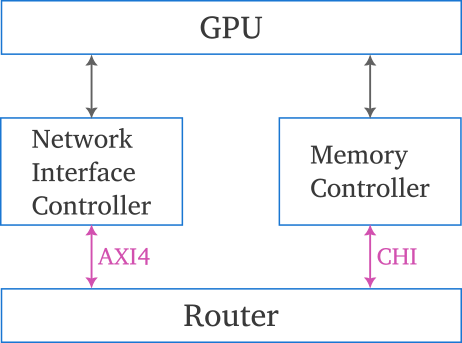
\includegraphics[width=0.7\linewidth]{images/component-architecture.png}
%    \caption{Nebula System Component Architecture}
%  \end{figure}
  \begin{itemize}
    \item Mesh topology generated by \texttt{nebula\_mesh\_top.sv}
    \item Routers interconnected, edge nodes terminated
    \item Each node: router + protocol bridge + GPU/memory interface
  \end{itemize}
  \hspace{5pt}
  \begin{figure}
	\centering
	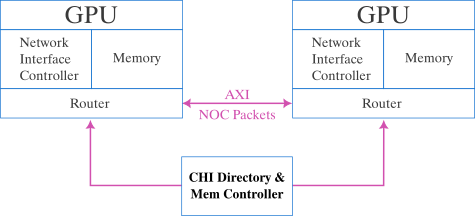
\includegraphics[width=0.6\linewidth]{images/inter-router-comms.png}
	\caption{Nebula Mesh Topology Example (4x4)}
  \end{figure}
  \note{
    	extbf{Mesh topology} is generated automatically by the \texttt{nebula\_mesh\_top.sv} module. Each node in the mesh contains a \textbf{router}, a \textbf{protocol bridge} (AXI/CHI), and a \textbf{GPU/memory interface}. \textbf{Edge nodes} are terminated with tie-off logic. The design supports \textbf{parameterizable mesh sizes} (2x2 to 8x8). Emphasize \textbf{modularity} and \textbf{scalability}.
  }
\end{frame}


%-------------------------------------------------
\begin{frame}{Node Connections}
	\begin{itemize}
		\item Nodes connect to their N, S, E \& W neighbours via bidirectional links.
		\item The links carry flit data, control signals, and credit information.
		\item 2D mesh architecture, scalable from 2x2 mesh to 8x8 mesh.
	\end{itemize}
	\hspace{5pt}
	\begin{figure}
		\centering
		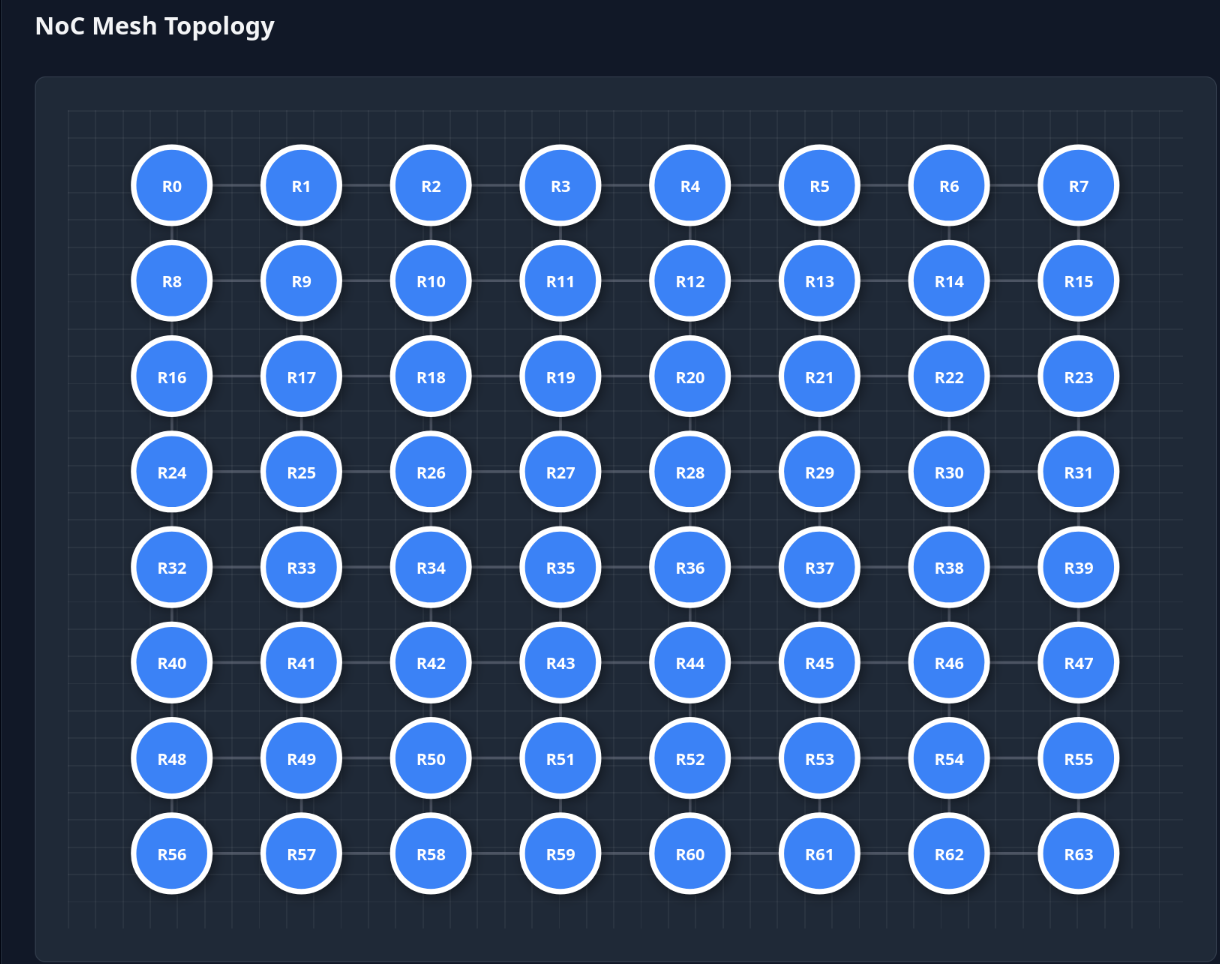
\includegraphics[width=0.4\linewidth]{images/router-mesh.png}
		\caption{Mesh Topology Example from Web Dashboard (8x8)}
	\end{figure}
\end{frame}

%-------------------------------------------------
\begin{frame}{Router Microarchitecture}
  \textbf{Five-Stage Pipeline:}
  \begin{enumerate}
    \item Buffer Write (BW): Input port, VC allocation
    \item Route Computation (RC): XY/adaptive routing
    \item Virtual Channel Allocation (VA): VC state machines, credit reservation
    \item Switch Allocation (SA): Crossbar arbitration, fairness
    \item Switch Traversal (ST): Data transmission, credit management
  \end{enumerate}
  \vspace{0.5em}
  \textbf{Features:}
  \begin{itemize}
    \item 4 VCs per port, 16-flit FIFO depth
    \item Credit-based flow control
    \item Round-robin arbitration
    \item Congestion-aware adaptive routing
  \end{itemize}
  \note{
    The \textbf{router} is implemented as a \textbf{five-stage pipeline}: \textbf{Buffer Write}, \textbf{Route Computation}, \textbf{Virtual Channel Allocation}, \textbf{Switch Allocation}, and \textbf{Switch Traversal}. Each stage is responsible for a specific part of the packet/flit journey. \textbf{Virtual channels} (VCs) and \textbf{credit-based flow control} prevent deadlock and buffer overflow. \textbf{Round-robin arbitration} ensures fairness. \textbf{Adaptive routing} uses congestion metrics to select optimal paths.
  }
\end{frame}

%-------------------------------------------------
\begin{frame}{Routing Algorithms}
  \begin{itemize}
    \item \textbf{XY Routing:} Dimension-ordered, deadlock-free
    \item \textbf{Adaptive Routing:} Congestion-aware, selects least congested path
    \item \textbf{Implementation:}
      \begin{itemize}
        \item Combinational logic compares router and destination coordinates
        \item Congestion metrics: buffer utilization, credit counts
        \item Programmable thresholds for adaptive switching
      \end{itemize}
  \end{itemize}
  \begin{block}{Technical Details}
    \begin{itemize}
      \item Route Computation: lines 260-380 in \texttt{nebula\_router.sv}
      \item VC Allocation: lines 630-690 in \texttt{nebula\_router.sv}
      \item Switch Allocation: lines 460-570 in \texttt{nebula\_router.sv}
    \end{itemize}
  \end{block}
  \note{
    	extbf{XY Routing} is a \textbf{dimension-ordered} algorithm that guarantees \textbf{deadlock freedom}. \textbf{Adaptive routing} uses \textbf{congestion metrics} (buffer utilization, credit counts) to select less congested paths. \textbf{Programmable thresholds} allow tuning of adaptive behavior. \textbf{Technical details} reference specific code lines for \textbf{route computation}, \textbf{VC allocation}, and \textbf{switch allocation}.
  }
\end{frame}

%-------------------------------------------------
\begin{frame}{Flit and Packet Format}
  \begin{itemize}
    \item \textbf{Flit:} 256 bits, defined in \texttt{nebula\_pkg.sv}
    \item \textbf{Header Fields:}
      \begin{itemize}
        \item Type (HEAD/BODY/TAIL/SINGLE)
        \item Source/Dest coordinates (4 bits each)
        \item VC ID (2 bits)
        \item Sequence number (16 bits)
        \item Packet ID (8 bits)
        \item QoS (4 bits)
        \item CRC (32 bits)
      \end{itemize}
    \item \textbf{Payload:} 208 bits
    \item \textbf{Multi-flit packets:} HEAD, BODY, TAIL; single-flit packets supported
  \end{itemize}
\end{frame}

%-------------------------------------------------
\begin{frame}{Protocol Translation Bridges}
  \begin{itemize}
    \item \textbf{AXI-NoC Bridge (\texttt{nebula\_axi\_noc\_bridge.sv}):}
      \begin{itemize}
        \item Burst decomposition, address mapping
        \item 64-entry reorder buffer
        \item Packet assembly/disassembly
        \item Error detection, latency monitoring
      \end{itemize}
    \item \textbf{CHI-NoC Bridge (\texttt{nebula\_chi\_noc\_bridge.sv}):}
      \begin{itemize}
        \item CHI message classification, VC mapping
        \item Directory-based MOESI coherency
        \item Snoop response aggregation
        \item Timeout/error handling
      \end{itemize}
    \item \textbf{Outstanding Transaction Management:}
      \begin{itemize}
        \item Hardware table tracks up to 64 operations
        \item Transaction ID, address, burst length, sequence, timeout
      \end{itemize}
  \end{itemize}
\end{frame}

%-------------------------------------------------
\begin{frame}{Packet Assembly and Disassembly}
  \begin{itemize}
    \item \textbf{Assembler (\texttt{nebula\_packet\_assembler.sv}):}
      \begin{itemize}
        \item Converts protocol transactions to flit packets
        \item Header generation, payload segmentation
        \item Address-to-coordinate mapping
      \end{itemize}
    \item \textbf{Disassembler (\texttt{nebula\_packet\_disassembler.sv}):}
      \begin{itemize}
        \item Reconstructs transactions from flits
        \item CRC verification, sequence management
        \item Handles out-of-order and multi-path delivery
      \end{itemize}
  \end{itemize}
\end{frame}

%-------------------------------------------------
\begin{frame}{Credit-Based Flow Control}
  \begin{itemize}
    \item \textbf{Credit Controller (\texttt{nebula\_credit\_flow\_ctrl.sv}):}
      \begin{itemize}
        \item Per-VC credit counters, max 16
        \item Increment on flit acceptance, decrement on allocation
        \item Prevents buffer overflow, deadlock
        \item \texttt{credits\_available} signals for arbitration
      \end{itemize}
    \item \textbf{Flow Control Protocol:}
      \begin{itemize}
        \item Sender stalls if credits = 0
        \item Lossless operation guaranteed
      \end{itemize}
  \end{itemize}
\end{frame}

%-------------------------------------------------
\begin{frame}{System Integration}
  \begin{itemize}
    \item \textbf{Top-Level Modules:}
      \begin{itemize}
        \item \texttt{nebula\_system\_top.sv}: Mesh instantiation, AXI4 interfaces, address mapping
        \item \texttt{nebula\_mesh\_top.sv}: Router grid generation, edge handling
        \item \texttt{nebula\_top.sv}: Configuration registers, system status, debug
      \end{itemize}
    \item \textbf{Address Mapping:}
      \begin{itemize}
        \item 64-bit global address space
        \item Static/dynamic schemes (partitioning, hashing)
        \item Hardware decoder for coordinate extraction
      \end{itemize}
    \item \textbf{Collective Operations:}
      \begin{itemize}
        \item Broadcast/multicast via packet replication
        \item Hardware barriers, reduction support
      \end{itemize}
  \end{itemize}
\end{frame}

%-------------------------------------------------
\begin{frame}{Verification and Testing}
  \begin{itemize}
    \item \textbf{RTL Testbenches (\texttt{code/tb/}):}
      \begin{itemize}
        \item Unit tests: packet assembler/disassembler, FIFO, arbiter
        \item Integration tests: AXI-NoC bridge, router, mesh
        \item System-level: end-to-end, multi-hop, congestion, performance
      \end{itemize}
    \item \textbf{Python Tools:}
      \begin{itemize}
        \item \texttt{nebula\_traffic\_generator.py}: Traffic pattern generation, testbench synthesis
        \item \texttt{nebula\_vcd\_parser.py}: VCD trace analysis, packet event extraction
      \end{itemize}
    \item \textbf{Metrics:}
      \begin{itemize}
        \item Latency, throughput, congestion, error rates
        \item Performance counters in routers and system top
      \end{itemize}
  \end{itemize}
\end{frame}

%-------------------------------------------------
\begin{frame}{Web Dashboard}
  \begin{itemize}
    \item \textbf{Backend:} Flask + Socket.IO (\texttt{web\_dashboard/backend/app.py})
    \item \textbf{Frontend:} Vanilla JS + Vite + Tailwind (\texttt{web\_dashboard/frontend/})
    \item \textbf{Features:}
      \begin{itemize}
        \item Real-time mesh visualization (SVG)
        \item Animated packet flows, congestion heatmap
        \item Performance metric graphing (utilization, latency, throughput)
        \item VCD trace replay, simulation control
        \item Traffic pattern selection (Uniform, Hotspot, CNN, Matrix, Transformer, etc.)
      \end{itemize}
    \item \textbf{Integration:}
      \begin{itemize}
        \item Runs Verilog simulations, parses VCD, updates UI via WebSocket
        \item API endpoints for mesh, performance, simulation control
      \end{itemize}
  \end{itemize}
\end{frame}

%-------------------------------------------------
\begin{frame}{Performance Monitoring}
  \begin{itemize}
    \item \textbf{Router-Level Counters:}
      \begin{itemize}
        \item Packets forwarded per direction
        \item Buffer utilization, VC statistics
        \item Congestion, temperature (simulated)
      \end{itemize}
    \item \textbf{System-Level Metrics:}
      \begin{itemize}
        \item Total packets routed, average latency, throughput
        \item Error and protocol violation tracking
        \item Historical trending for optimization
      \end{itemize}
    \item \textbf{Visualization:}
      \begin{itemize}
        \item Time-series graphs, mesh overlays
        \item VCD replay for cycle-accurate analysis
      \end{itemize}
  \end{itemize}
\end{frame}

%-------------------------------------------------
\begin{frame}{Technical Challenges}
  \begin{itemize}
    \item \textbf{Scalability:} Mesh generation, address mapping for large grids
    \item \textbf{Coherency:} CHI protocol edge cases, directory state management
    \item \textbf{Adaptive Routing:} Congestion metrics, deadlock avoidance
    \item \textbf{Verification:} Multi-level test coverage, error injection
    \item \textbf{Integration:} Protocol bridge correctness, performance counter aggregation
    \item \textbf{Visualization:} Real-time updates, VCD parsing, UI responsiveness
  \end{itemize}
\end{frame}

%-------------------------------------------------
\begin{frame}{Current Status and Future Work}
  \begin{itemize}
    \item \textbf{Completed:}
      \begin{itemize}
        \item Mesh topology, router pipeline, protocol bridges
        \item AXI4/CHI support, packet assembler/disassembler
        \item Python traffic generator, VCD parser, web dashboard
        \item Verification infrastructure, performance monitoring
      \end{itemize}
    \item \textbf{In Progress:}
      \begin{itemize}
        \item Advanced adaptive routing, QoS features
        \item Hierarchical clustering, multi-mesh support
        \item Enhanced CHI edge case handling
        \item Dashboard UI improvements, analytics
      \end{itemize}
    \item \textbf{Planned:}
      \begin{itemize}
        \item FPGA prototyping, hardware deployment
        \item Deep learning workload benchmarks
        \item Fault tolerance, dynamic reconfiguration
      \end{itemize}
  \end{itemize}
\end{frame}

%-------------------------------------------------
\begin{frame}{References}
  \begin{itemize}
    \item SystemVerilog RTL: \texttt{code/rtl/}
    \item Python Tools: \texttt{code/python/}
    \item Testbenches: \texttt{code/tb/}
    \item Documentation: \texttt{docs/final\_report.tex}, \texttt{docs/abstract.tex}
    \item Dashboard: \texttt{web\_dashboard/}
  \end{itemize}
\end{frame}

%-------------------------------------------------
\begin{frame}{Q\&A}
  \centering
  \Huge Questions?
\end{frame}

%-------------------------------------------------
\begin{frame}{Nebula RTL Modules: Overview}
  \begin{itemize}
    \item The Nebula NoC is composed of modular, parameterized SystemVerilog RTL blocks.
    \item Each module is designed for scalability, protocol flexibility, and high throughput.
    \item This section details the design decisions, code structure, and unique features of each RTL module.
  \end{itemize}
\end{frame}

%-------------------------------------------------
\begin{frame}{nebula\_top.sv: System Integration (1/2)}
  \textbf{Design Decisions:}
  \begin{itemize}
    \item Parameterized mesh size, protocol enable/disable, and config bus widths.
    \item Unified configuration and status interface for software control.
    \item Modular instantiation of routers, bridges, and monitoring logic.
  \end{itemize}
  \textbf{Key Code:}
  \begin{itemize}
    \item Parameter and function definitions for mesh configuration.
    \item Synchronous logic for system control and status.
  \end{itemize}
\end{frame}

%-------------------------------------------------
\begin{frame}{nebula\_top.sv: System Integration (2/2)}
  \textbf{Cool Features:}
  \begin{itemize}
    \item System-wide error aggregation and debug trace export.
    \item Performance counters and status registers for real-time monitoring.
    \item Generate blocks for scalable instantiation.
  \end{itemize}
  \textbf{Key Code:}
  \begin{itemize}
    \item Generate loops for node instantiation.
    \item Status aggregation logic.
  \end{itemize}
\end{frame}

%-------------------------------------------------
\begin{frame}{nebula\_system\_top.sv: System-Level Integration (1/2)}
  \textbf{Design Decisions:}
  \begin{itemize}
    \item Centralizes mesh, memory, and protocol bridge instantiation.
    \item Implements global address decoding and mapping.
    \item Coordinates system resets and status propagation.
  \end{itemize}
  \textbf{Key Code:}
  \begin{itemize}
    \item Mesh instantiation with parameterized width and height.
    \item Address mapping logic from global to local address space.
  \end{itemize}
\end{frame}

%-------------------------------------------------
\begin{frame}{nebula\_system\_top.sv: System-Level Integration (2/2)}
  \textbf{Cool Features:}
  \begin{itemize}
    \item Flexible address mapping for heterogeneous memory systems.
    \item System-level reset and error handling.
    \item Integration hooks for simulation and testbench control.
  \end{itemize}
  \textbf{Key Code:}
  \begin{itemize}
    \item Synchronous reset and control logic.
    \item Error status propagation and handling.
  \end{itemize}
\end{frame}

%-------------------------------------------------
\begin{frame}{nebula\_mesh\_top.sv: Mesh Topology (1/2)}
  \textbf{Design Decisions:}
  \begin{itemize}
    \item 2D grid instantiation using nested generate loops.
    \item Edge node handling (tie-off or wrap-around).
    \item Parameterized for mesh width/height.
  \end{itemize}
  \textbf{Key Code:}
  \begin{itemize}
    \item Generate loops for X and Y dimensions of the mesh.
    \item Conditional logic for edge node connections.
  \end{itemize}
\end{frame}

%-------------------------------------------------
\begin{frame}{nebula\_mesh\_top.sv: Mesh Topology (2/2)}
  \textbf{Cool Features:}
  \begin{itemize}
    \item Automated port wiring for all mesh neighbors.
    \item Edge detection logic for boundary nodes.
    \item Supports mesh reconfiguration for fault tolerance.
  \end{itemize}
  \textbf{Key Code:}
  \begin{itemize}
    \item Port connection logic using generate and if-else constructs.
    \item Tie-off or wrap-around logic for edge cases.
  \end{itemize}
\end{frame}

%-------------------------------------------------
\begin{frame}{nebula\_router.sv: Router Pipeline (1/2)}
  \textbf{Design Decisions:}
  \begin{itemize}
    \item Five-stage pipeline for high throughput.
    \item Virtual channel allocation and credit-based flow control.
    \item Adaptive and deterministic routing support.
  \end{itemize}
  \textbf{Key Code:}
  \begin{itemize}
    \item Synchronous logic for each stage of the router pipeline.
    \item Combinational logic for route computation and switch allocation.
  \end{itemize}
\end{frame}

%-------------------------------------------------
\begin{frame}{nebula\_router.sv: Router Pipeline (2/2)}
  \textbf{Cool Features:}
  \begin{itemize}
    \item Per-port and per-VC performance counters.
    \item Error detection for buffer overflow and protocol violations.
    \item Round-robin arbitration for switch allocation.
  \end{itemize}
  \textbf{Key Code:}
  \begin{itemize}
    \item Performance counter increment and error flag logic.
    \item Arbitration logic for switch allocation.
  \end{itemize}
\end{frame}

%-------------------------------------------------
\begin{frame}{nebula\_axi\_if.sv: AXI4 Interface (1/2)}
  \textbf{Design Decisions:}
  \begin{itemize}
    \item Parameterized AXI widths for flexible integration.
    \item FIFO-based buffering for all AXI channels.
    \item Clock domain crossing support.
  \end{itemize}
  \textbf{Key Code:}
  \begin{itemize}
    \item AXI signal assignments and FIFO push/pop logic.
    \item Clock domain crossing synchronizers.
  \end{itemize}
\end{frame}

%-------------------------------------------------
\begin{frame}{nebula\_axi\_if.sv: AXI4 Interface (2/2)}
  \textbf{Cool Features:}
  \begin{itemize}
    \item AXI burst handling and response reordering.
    \item Backpressure propagation to the NoC.
    \item Error injection for verification.
  \end{itemize}
  \textbf{Key Code:}
  \begin{itemize}
    \item Logic for burst-to-packet conversion and response assembly.
    \item Error detection and handling logic.
  \end{itemize}
\end{frame}

%-------------------------------------------------
\begin{frame}{nebula\_axi\_noc\_bridge.sv: AXI4-NoC Bridge (1/2)}
  \textbf{Design Decisions:}
  \begin{itemize}
    \item Decomposes AXI bursts into NoC packets.
    \item Maintains reorder buffer for out-of-order responses.
    \item Tracks outstanding transactions by ID.
  \end{itemize}
  \textbf{Key Code:}
  \begin{itemize}
    \item Logic for AXI to NoC packet conversion.
    \item Reorder buffer management for response assembly.
  \end{itemize}
\end{frame}

%-------------------------------------------------
\begin{frame}{nebula\_axi\_noc\_bridge.sv: AXI4-NoC Bridge (2/2)}
  \textbf{Cool Features:}
  \begin{itemize}
    \item Out-of-order response assembly from NoC flits.
    \item Error detection and reporting for protocol violations.
    \item Latency monitoring for each transaction.
  \end{itemize}
  \textbf{Key Code:}
  \begin{itemize}
    \item Logic for assembling responses from NoC flits.
    \item Error and latency monitoring logic.
  \end{itemize}
\end{frame}

%-------------------------------------------------
\begin{frame}{nebula\_chi\_interface.sv: CHI Protocol (1/2)}
  \textbf{Design Decisions:}
  \begin{itemize}
    \item Implements CHI request, response, and data channels.
    \item State machine for protocol sequencing.
    \item Snoop and directory support.
  \end{itemize}
  \textbf{Key Code:}
  \begin{itemize}
    \item CHI protocol state machine implementation.
    \item Logic for handling CHI requests and responses.
  \end{itemize}
\end{frame}

%-------------------------------------------------
\begin{frame}{nebula\_chi\_interface.sv: CHI Protocol (2/2)}
  \textbf{Cool Features:}
  \begin{itemize}
    \item FIFO-based buffering for all CHI channels.
    \item Protocol error detection and recovery.
    \item Integration with directory and snoop logic.
  \end{itemize}
  \textbf{Key Code:}
  \begin{itemize}
    \item Buffer management logic for CHI channels.
    \item Error handling and recovery logic.
  \end{itemize}
\end{frame}

%-------------------------------------------------
\begin{frame}{nebula\_chi\_noc\_bridge.sv: CHI-NoC Bridge (1/2)}
  \textbf{Design Decisions:}
  \begin{itemize}
    \item Maps CHI message types to NoC VCs.
    \item Handles coherency, snoop, and directory state transitions.
    \item Aggregates snoop responses and manages timeouts.
  \end{itemize}
  \textbf{Key Code:}
  \begin{itemize}
    \item Logic for mapping CHI messages to NoC virtual channels.
    \item Snoop response aggregation and timeout handling logic.
  \end{itemize}
\end{frame}

%-------------------------------------------------
\begin{frame}{nebula\_chi\_noc\_bridge.sv: CHI-NoC Bridge (2/2)}
  \textbf{Cool Features:}
  \begin{itemize}
    \item Timeout detection for snoop responses.
    \item Priority mapping for CHI traffic classes.
    \item Error handling for protocol mismatches.
  \end{itemize}
  \textbf{Key Code:}
  \begin{itemize}
    \item Timeout detection and handling logic.
    \item Priority encoding logic for CHI messages.
  \end{itemize}
\end{frame}

%-------------------------------------------------
\begin{frame}{nebula\_chi\_directory.sv: Directory Controller (1/2)}
  \textbf{Design Decisions:}
  \begin{itemize}
    \item Implements MOESI directory for cache coherency.
    \item Handles snoop requests and state transitions.
    \item Manages race conditions and protocol corner cases.
  \end{itemize}
  \textbf{Key Code:}
  \begin{itemize}
    \item Directory state machine implementation for MOESI.
    \item Logic for handling snoop requests and responses.
  \end{itemize}
\end{frame}

%-------------------------------------------------
\begin{frame}{nebula\_chi\_directory.sv: Directory Controller (2/2)}
  \textbf{Cool Features:}
  \begin{itemize}
    \item MOESI state machine for each cache line.
    \item Snoop response aggregation and forwarding.
    \item Error detection for invalid state transitions.
  \end{itemize}
  \textbf{Key Code:}
  \begin{itemize}
    \item State transition logic for MOESI protocol.
    \item Logic for aggregating and forwarding snoop responses.
  \end{itemize}
\end{frame}

%-------------------------------------------------
\begin{frame}{nebula\_niu\_axi.sv: AXI NIU (1/2)}
  \textbf{Design Decisions:}
  \begin{itemize}
    \item Buffers and arbitrates between protocol and NoC domains.
    \item Handles packetization and depacketization.
    \item Manages local error and status reporting.
  \end{itemize}
  \textbf{Key Code:}
  \begin{itemize}
    \item Logic for buffering and arbitration between AXI and NoC.
    \item Packetization and depacketization logic.
  \end{itemize}
\end{frame}

%-------------------------------------------------
\begin{frame}{nebula\_niu\_axi.sv: AXI NIU (2/2)}
  \textbf{Cool Features:}
  \begin{itemize}
    \item Local error detection and reporting.
    \item Arbitration between multiple protocol sources.
    \item Parameterized for different AXI widths.
  \end{itemize}
\end{frame}

%-------------------------------------------------
\begin{frame}{nebula\_packet\_assembler.sv: Packet Assembly (1/2)}
  \textbf{Design Decisions:}
  \begin{itemize}
    \item Converts protocol transactions to NoC flit packets.
    \item Segments payloads across multiple flits.
    \item Generates flit headers with CRC and sequence info.
  \end{itemize}
  \textbf{Key Code:}
  \begin{itemize}
    \item Header construction logic for different packet types.
    \item Payload segmentation and CRC generation logic.
  \end{itemize}
\end{frame}

%-------------------------------------------------
\begin{frame}{nebula\_packet\_assembler.sv: Packet Assembly (2/2)}
  \textbf{Cool Features:}
  \begin{itemize}
    \item Address-to-coordinate mapping for mesh routing.
    \item CRC generation for each packet.
    \item Handles both single-flit and multi-flit packets.
  \end{itemize}
\end{frame}

%-------------------------------------------------
\begin{frame}{nebula\_packet\_disassembler.sv: Packet Disassembly (1/2)}
  \textbf{Design Decisions:}
  \begin{itemize}
    \item Reconstructs protocol transactions from flits.
    \item Verifies CRC and sequence numbers.
    \item Handles out-of-order and multi-path delivery.
  \end{itemize}
  \textbf{Key Code:}
  \begin{itemize}
    \item Logic for reassembling transactions from received flits.
    \item CRC verification and error handling logic.
  \end{itemize}
\end{frame}

%-------------------------------------------------
\begin{frame}{nebula\_packet\_disassembler.sv: Packet Disassembly (2/2)}
  \textbf{Cool Features:}
  \begin{itemize}
    \item Out-of-order packet reassembly.
    \item Error flagging for CRC mismatches.
    \item Sequence number tracking for reliability.
  \end{itemize}
\end{frame}

%-------------------------------------------------
\begin{frame}{nebula\_pkg.sv: Global Package (1/2)}
  \textbf{Design Decisions:}
  \begin{itemize}
    \item Centralizes all parameter, type, and enum definitions.
    \item Ensures consistency across all modules.
    \item Provides utility functions for coordinate mapping, CRC, etc.
  \end{itemize}
  \textbf{Key Code:}
  \begin{itemize}
    \item Parameter and type definitions for NoC and protocol.
    \item Utility function implementations (e.g., CRC calculation).
  \end{itemize}
\end{frame}

%-------------------------------------------------
\begin{frame}{nebula\_pkg.sv: Global Package (2/2)}
  \textbf{Cool Features:}
  \begin{itemize}
    \item Parameterized mesh and flit widths.
    \item Strong type safety for protocol and NoC structures.
    \item Utility functions for address/coordinate conversion.
  \end{itemize}
\end{frame}

%-------------------------------------------------
\begin{frame}{nebula\_top\_simple.sv: Minimal Top (1/2)}
  \textbf{Design Decisions:}
  \begin{itemize}
    \item Minimal mesh and protocol integration for bring-up.
    \item Used for unit and smoke tests.
  \end{itemize}
  \textbf{Key Code:}
  \begin{itemize}
    \item Minimal mesh instantiation and AXI interface.
    \item Basic configuration and status logic.
  \end{itemize}
\end{frame}

%-------------------------------------------------
\begin{frame}{nebula\_top\_simple.sv: Minimal Top (2/2)}
  \textbf{Cool Features:}
  \begin{itemize}
    \item Fast simulation for basic connectivity checks.
    \item Easy to extend for new protocol bridges.
  \end{itemize}
\end{frame}

%-------------------------------------------------
\begin{frame}{common/: Reusable Modules (1/2)}
  \textbf{Design Decisions:}
  \begin{itemize}
    \item Implements core NoC utilities: CRC, FIFO, credit flow, arbitration.
    \item Parameterized for width, depth, and protocol.
  \end{itemize}
  \textbf{Key Code:}
  \begin{itemize}
    \item CRC calculation function and FIFO module.
    \item Credit flow control and round-robin arbiter.
  \end{itemize}
\end{frame}

%-------------------------------------------------
\begin{frame}{common/: Reusable Modules (2/2)}
  \textbf{Cool Features:}
  \begin{itemize}
    \item Round-robin arbitration for fairness.
    \item Parameterized FIFO for flit/packet buffering.
    \item Modular, reusable code for all NoC blocks.
  \end{itemize}
  \textbf{Key Code:}
  \begin{itemize}
    \item Generic FIFO read/write logic.
    \item Arbiter grant and request handling.
  \end{itemize}
\end{frame}

\end{document}
